%!TEX root = book.tex

\chapter{Hydrostatic Equilibrium}

Looking forward, we will shortly need to determine the non-grey opacity of matterin a stellar atmosphere. We will do this first under the assumption of LTE, and the calculation will have as parameters the given composition, the temperature, and the density. The temperature can be obtained from the requirement for thermal equilibrium, but up to this point we have nothing to constrain the density. In this chapter, we will address that shortcoming.

\newslide

\section{Mechanical Equilibrium}

We often assume that stellar atmospheres are in mechanical equilibrium, with no net force on each element of gas. If they were even slightly out of mechanical equilibrium, they would rapidly expand or collapse on a timescale comparable to the free-fall time or sound-crossing time; for the Sun this is about half an hour.

Of course, there is a part of a star that does expand rapidly -- the wind -- and there are stars that pulsate, but assuming mechanical equilibrium is a good approximation for most photospheres.

\newslide

\section{Hydrostatic Equilibrium}

The dominant forces in a stellar atmosphere are gravity and pressure. Thus, mechanical equilibrium requires balancing the inwards force of gravity and the outwards pressure force. This special case of mechanical equilibrium is known as hydrostatic equilibrium.

\begin{figure}
\begin{center}
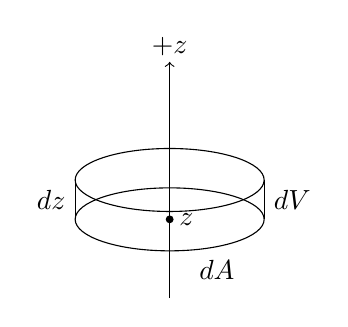
\begin{tikzpicture}
\fill[black] (0,0) circle [radius=0.05];
\draw[->] (0,-1) -- (0,2);
\draw(0,0) ellipse [x radius=1.2cm,y radius=0.4cm];
\draw(0,0.5) ellipse [x radius=1.2cm,y radius=0.4cm];
\draw(+1.2,0.5) -- (+1.2,0);
\draw(-1.2,0.5) -- (-1.2,0);
\draw (0,2.2) node {$+z$};
\draw (0,0) node[right] {$z$};
\draw (1.2,0.25) node[right] {$dV$};
\draw (0.6,-0.4) node[below] {$dA$};
\draw (-1.2,0.25) node[left] {$dz$};
\end{tikzpicture}
\end{center}
\caption{The geometry used in the derivation of the equation of hydrostatic equilibrium.}
\label{fig-hydrostatic-equilibrium}
\end{figure}

We will now determine the condition of hydrostatic equilibrium in plane-parallel geometry. Consider an element of gas whose volume is $dV$. This volume is constructed by translating an area $dA$ perpendicular to the $z$ axis a distance $dz$.

The inwards force of gravity on the element is 
\begin{align}
\rho g dV
\end{align}
in which $\rho$ is the density and $g$ is the gravitational acceleration towards the center of the star.
The outwards pressure force on the element is
\begin{align}
P(z)dA - P(z+dz)dA,
\end{align}
in which $P$ is the pressure, and the first term is the upwards force on the lower surface of the volume and the second term is the downwards force on the upper surface of the volume. In hydrostatic equilibrium, these must balance, and we have
\begin{align}
P(z)dA - P(z+dz)dA = \rho g dV.
\end{align}
Expanding $P$ for small $dz$ gives
\begin{align}
P(z)dA - \left[P(z) + dz \frac{dP}{dz}\right] dA = \rho g dV,
\end{align}
or
\begin{align}
\frac{dP}{dz} = -\rho g.
\label{equation:hydrostatic-equilibrium}
\end{align}
This is known as the equation of hydrostatic equilibrium. Note that since $\rho$ and $g$ are positive, $dP/dz$ is negative and the pressure must decrease outwards with $z$.

We often assume that the atmosphere is thin compared to the radius of the star, so the gravity does not change significantly within the atmosphere. That is, we assume that $g$ is a constant equal to the surface gravity $GM_*/R_*^2$

\newslide

\subsection{The Equation of State}

The pressure that provides support against gravity is a combination of gas and radiation pressure. (In this context, by “pressure” we do mean “force per unit area” rather than “momentum flux”.) The radiation pressure can be very important in hot stars and evolved stars, but for the moment we will ignore it and assume that the pressure is dominated by gas pressure.

For an ideal gas, the density and pressure are given by
\begin{align}
\rho &= n\mu \mH\\
\intertext{and}
P &= nkT\\
&= \frac{\rho kT}{\mu \mH}.
\end{align}
in which $n$ is the particle density, $\rho$ is the mass density, $\mu$ is the mean molecular mass, and $\mH$ is the mass of the proton. Thus, we see that the increase in pressure with depth can be provided by an increase in temperature, an increase in density, or a decrease in mean molecular mass (through increasing ionization). It’s typically a combination of all three.

\newslide

\subsection{The Pressure Scale Height}

If we divide the equation of hydrostatic equilibrium on both sides by the pressure, we obtain
\begin{align}
\frac{1}{P} \frac{dP}{dz} = \frac{d\ln P}{dz} = -\frac{\rho g}{P} \equiv -\frac{1}{H}.
\label{equation:scale-height}
\end{align}
This defines the pressure scale height $H \equiv P/\rho g$, the characteristic distance for changes in the relative pressure. 

As we can see, the pressure scale height depends on the equation of state -- the relation between pressure and density -- for the material and on the surface gravity. For an ideal gas, we have
\begin{align}
H = \frac{kT}{\mu \mH g}.
\end{align}
Since $T/\mu$ will in general not be constant in a real atmosphere, $H$ will also not be constant and so we normally cannot integrate $d\ln P/dz = 1/H$ directly.

We can obtain a slightly different form of the equation of hydrostatic equilibrium by dividing equation \ref{equation:scale-height} by $-\chi$, obtaining
\begin{align}
\frac{d\ln P}{d\tau} = \frac{1}{\chi H} = \frac{l}{H}.
\end{align}
Thus, we see that the ratio of the mean free path for a photon $l$ to the pressure scale height $l$ defines the scale of the relative change in the pressure per unit optical depth. If $l/H$ is large, the pressure changes dramatically, whereas if $l/H$ is small, the change is less significant.

The pressure scale height in the solar atmosphere at the point that $T = \Teff$ is about 140 km. On the other hand, the physical extent of the solar atmosphere is about 1000 km. Thus, we should expect that in the Sun the pressure does change dramatically through the solar atmosphere.

%Expanding $P$ in terms of density, temperature, and mean molecular mass, we find
%\begin{align}
%\frac{1}{\rho}\frac{d\rho}{dz} + \frac{1}{T}\frac{dT}{dz} - \frac{1}{\mu}\frac{d\mu}{dz}&= -\frac{1}{H}.
%\label{equation:hydrostatic-equilibrium-logarithmic}
%\end{align}
%and
%\begin{align}
%\frac{1}{\rho}\frac{d\rho}{d\tau} + \frac{1}{T}\frac{dT}{d\tau} - \frac{1}{\mu}\frac{d\mu}{d\tau}= \frac{l}{H}.
%\label{equation:hydrostatic-equilibrium-logarithmic}
%\end{align}

\newslide

\section{The Constant Scale-Height Atmosphere}

Let’s start by considering an atmosphere with a constant scale height. If $H$ is constant, we can integrate $d\ln P/dz = 1/H$ directly to give
\begin{align}
P = P_0 e^{-(z-z_0)/H},
\end{align}
in which we have applied an arbitrary boundary condition that $P(z_0) = P_0$. We see that pressure increases exponentially inwards. Each time the depth into the atmosphere increases by $H$, the pressure rises by a factor of $e$.

One theoretical example of a constant scale-height atmosphere is an isothermal atmosphere ($dT/dz = 0$) with a constant molecular mass ($d\mu/dz = 0$). This is approximately appropriate for the lower atmosphere of the Earth, but not for a stellar atmosphere.

%\section{Grey Atmosphere in LTE}
%
%In a grey atmosphere in LTE, the temperature increases with depth. Thus, we would expect the density to increase less quickly than exponentially, since the increasing temperature makes some contribution to the increasing pressure.
%
%For a grey atmosphere, we have
%\begin{align}
%T^4 = \frac{3}{4}\Teff^4 \left(\tau + q\right),
%\end{align}
%and so
%\begin{align}
%\frac{1}{T}\frac{dT}{d\tau} 
%&= \frac{3\Teff^4}{16 T^4} \left(1 + \frac{dq}{d\tau}\right)\\
%&=\frac{1}{4}\left(\frac{1+\frac{dq}{d\tau}}{\tau+q}\right).
%\end{align}
%Furthermore, we have
%\begin{align}
%\frac{l}{H} &= \frac{l\mu\mH g}{kT}\\
%&=\left(\frac{4}{3(\tau+q)}\right)^{1/4}\frac{l\mu\mH g}{k\Teff}.
%\end{align}
%If $\mu$ and $g$ are constant through the atmosphere, then we can define $\Heff \equiv {k\Teff}/{\mu\mH g}$ and write this as
%\begin{align}
%\frac{l}{H} &= \left(\frac{4}{3(\tau+q)}\right)^{1/4}\frac{l}{\Heff}.
%\end{align}
%If we assume that $\chi$ is a power-law in $\rho$, then
%
%In order to obtain $dT/dz$, we must use $d\tau \equiv -\chi dz$, which gives
%\begin{align}
%\frac{1}{T}\frac{dT}{dz} = -\frac{3\Teff^4\chi}{16T^4}\left(1 + \frac {dq}{d\tau}\right).
%\end{align}
%If we assume that $\chi = \chi_0 (\rho/\rho_0)^\alpha$, then
%\begin{align}
%\frac{1}{T}\frac{dT}{dz} = -\frac{3\Teff^4\chi_0 \rho^\alpha}{16T^4\rho_0^\alpha}\left(1 + \frac {dq}{d\tau}\right).
%\end{align}
%Equation \ref{equation:hydrostatic-equilibrium-logarithmic} then becomes
%\begin{align}
%\frac{1}{\rho}\frac{d\rho}{dz} -\frac{3\Teff^4\chi_0 \rho^\alpha}{16T^4\rho_0^\alpha}\left(1 + \frac {dq}{d\tau}\right) = -\frac{1}{H}.
%\end{align}


\newslide

\section{The Grey Atmosphere}

\begin{figure}
\footnotesize
\begin{tikzpicture}
\begin{axis}[
   xlabel={$\tau$},
   ylabel={$T(\tau)/T(1)$ or $\rho(\tau)/\rho(1)$},
   ymin=0.0,
   ymax=3,
   minor y tick num=3,
   xmin=0,
   xmax=3,
   minor x tick num=4,
]
\addplot[black,solid] table[x index=0,y index=1]{chapter-6/grey-density.tsv};
\addplot[black,dashed] table[x index=0,y index=2]{chapter-6/grey-density.tsv};
\addplot[black,dotted] table[x index=0,y index=0]{chapter-6/grey-density.tsv};
\end{axis}
\end{tikzpicture}
\caption{The value of $T(\tau)/T(1)$ (solid line) and $\rho(\tau)/\rho(1)$ (dashed line) for an LTE grey atmosphere with constant $\mu$ and $a$. The value of $\rho(\tau)/\rho(1)$ for an isothermal atmosphere is shown as a dotted line.}
\label{figure:grey-density}
\end{figure}

In a grey atmosphere in LTE and in the absence of scattering, the temperature increases with depth as
\begin{align}
T^4 = \frac{3}{4}T_\mathrm{eff}^4[\tau + q(\tau)].
\end{align}
Thus, we would expect the density to increase less quickly than exponentially, since the increasing temperature makes some contribution to the increasing pressure.

We adopted the plane-parallel approximation by assuming that the atmosphere was thin compared to the radius of the star. Given this, we can also assume that the surface gravity $g \equiv GM/R^2$ is constant. 

The condition of hydrostatic equilibrium requires
\begin{align}
\frac{dP}{dz} = -\rho g.
\end{align}
Dividing by $d\tau/dz=-\chi$, we find
\begin{align}
\frac{dP}{d\tau} = \left(\frac{\rho}{\chi}\right)g.
\end{align}
If we write $\rho$ and $\chi$ in terms of the mean molecular mass $\mu$ and the mean cross-section $a$ using $\rho = \mu m_\mathrm{H} n$ and $\chi = a n$, we obtain
\begin{align}
\frac{dP}{d\tau} = \left(\frac{\mu }{a}\right)m_\mathrm{H}g.
\end{align}
For simplicity, we will now assume that $\mu$ and $a$ are constant in the atmosphere, in which case we can integrate to obtain
\begin{align}
P(\tau) = \left(\frac{\mu}{a}\right) m_\mathrm{H}g\tau + P(0).
\end{align}
At the surface of the atmosphere, the density must tend to zero, and so $P(0)$ must also tend to zero. Thus,
\begin{align}
P(\tau) = \left(\frac{\mu}{a}\right)m_\mathrm{H}g\tau.
\end{align}
We see that in this atmosphere, the pressure rises roughly linearly with $\tau$ and, moreover, roughly linearly with the surface gravity $g$.

The density is given by
\begin{align}
n(\tau) = \frac{P}{kT}.
\end{align}
Substituting for the temperature in a grey atmosphere, we obtain
\begin{align}
n(\tau) = \left(\frac43\right)^{1/4}\left(\frac{\mu m_\mathrm{H}}{a kT_\mathrm{eff}}\right) g\tau\left[\tau + q(\tau)\right]^{-1/4}.
\end{align}
For $\tau\ll1$, $\tau + q(\tau)\approx q(0)$ and so the dependence on $\tau$ is linear. For $\tau \gg 1$, $\tau + q(\tau) \approx \tau$ and so the dependence changes to $\tau^{3/4}$. The exact behaviour of $T$ and $\rho$ are shown in Figure~\ref{figure:grey-density}. Throughout the atmosphere, though, the density increases with $\tau$. Moreover, the density at a given $\tau$ depends linearly on the surface gravity.

It’s worth comparing this result for the grey atmosphere with the result for an isothermal atmosphere with the same restrictions on $\mu$ and $a$. In this case, we would have found that $P \propto \tau$. This is also shown in Figure~\ref{figure:grey-density}. We see that the grey atmosphere is quite close to the isothermal atmosphere until $\tau$ becomes large and the increasing temperature begins to slow the increase in density.

Real atmospheres are not grey and do not have constant molecular masses and mean cross-sections. Nevertheless, real atmospheres show these tendencies: the density increases with $\tau$ in a given atmosphere and the density increases with increasing $g$ at a given $\tau$. 

\newslide

\subsection{Surface Gravity}

We have seen that the surface gravity $g = GM_*/R_*^2$ has a crucial role in determining the density in an atmosphere. The surface gravity is conventionally given as $\log g$, the base-10 logarithm of $g$ in $\mathrm{cm\,s^{-2}}$. Dwarfs stars (luminosity class V) typically have surface gravities of 4.0 to 4.6, giant stars (luminosity class III) have typical surface gravities from 3.8 to 1.7, and supergiant stars (luminosity class Ib) have typical surface gravities from 2.0 to 0.7. Thus, dwarfs typically have denser atmospheres than giants and giants typically have denser atmospheres than supergiants.

